% Figure 3: Ground-Plane Projection Geometry with Pitch/Roll Compensation (Monochrome 300 DPI)
\begin{figure}[!t]
\centering
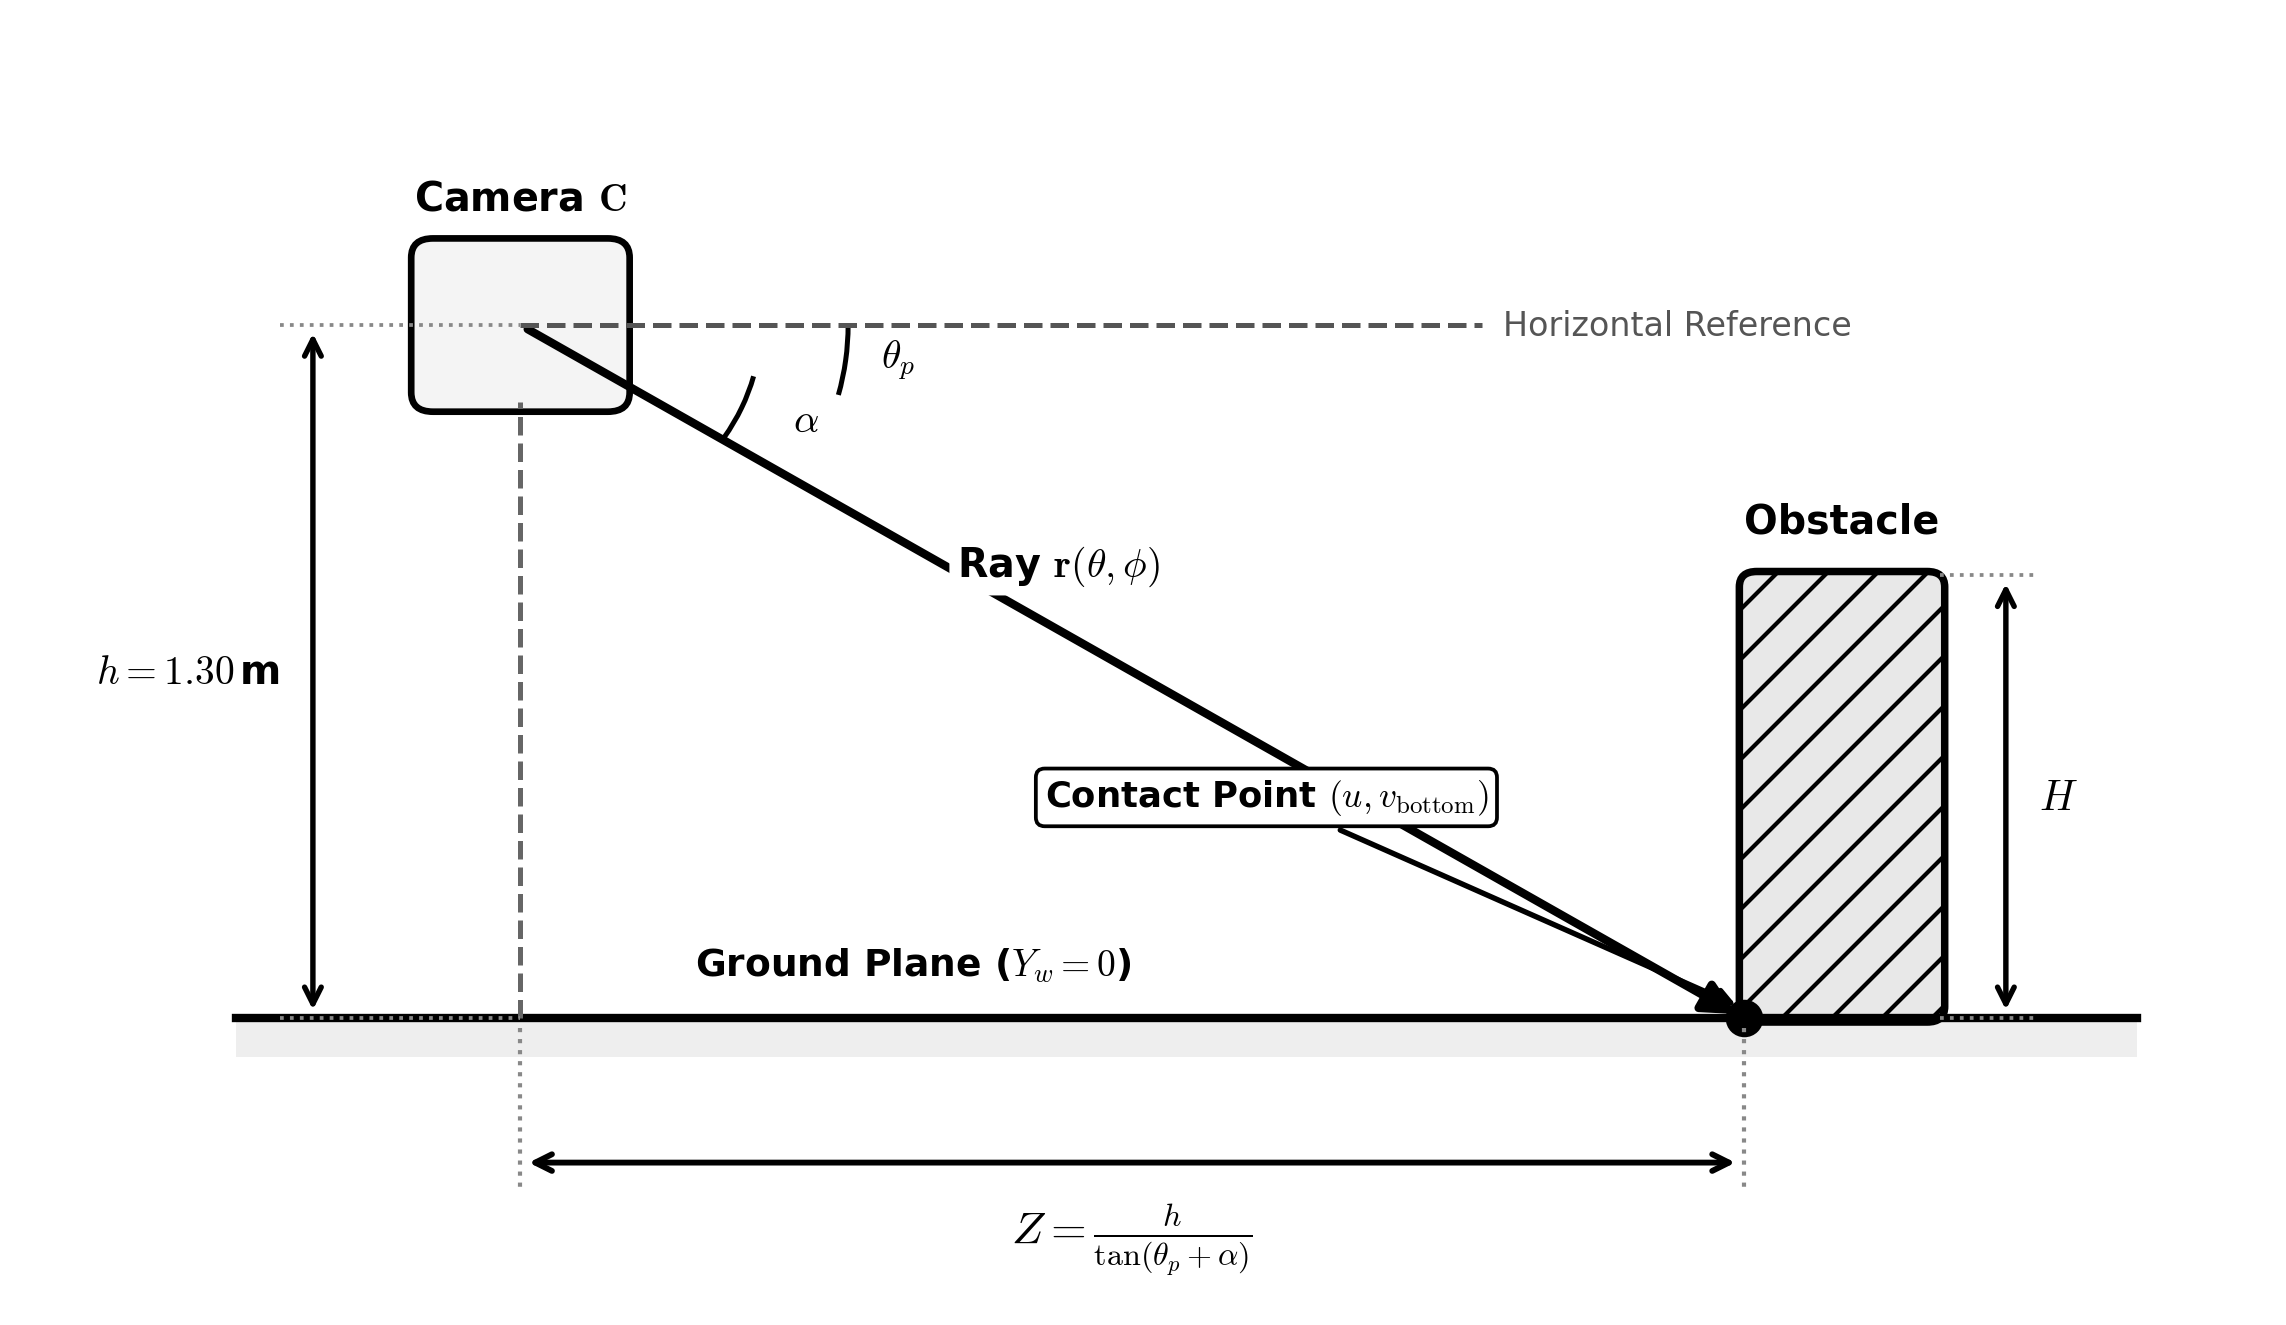
\includegraphics[width=\columnwidth]{figures/fig_projection.png}
\caption{Monocular ground-plane inverse ray projection geometry (black and white): bottom contact point $(u, v_{\text{bottom}})$ is projected onto ground plane $Y_w = 0$ incorporating IMU pitch $\theta_p$ and roll $\phi$ to recover metric distance $Z$, lateral offset $X$, and obstacle height $H$.}
\label{fig:ground_projection_geometry}
\end{figure}
